% 判定 3：一组对边平行且相等 → 平行四边形
\documentclass[tikz,border=4pt]{standalone}
\usepackage{ctex}
\usepackage{amsmath}
\usetikzlibrary{calc, decorations.markings, arrows.meta}
\begin{document}
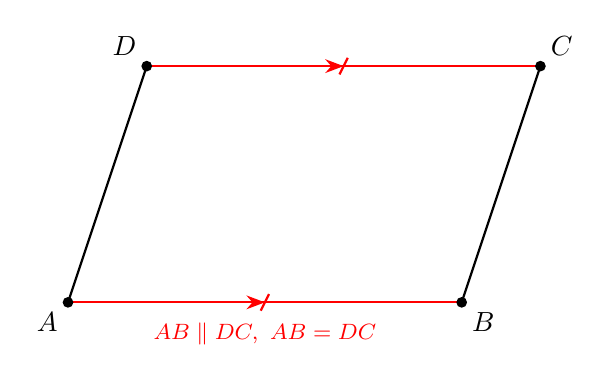
\begin{tikzpicture}[scale=1.0, thick,
  tickone/.style={postaction={decorate, decoration={markings,
    mark=at position 0.5 with {\draw (-1.5pt,-3pt) -- (1.5pt,3pt);}}}},
  arrowone/.style={postaction={decorate, decoration={markings,
    mark=at position 0.5 with {\arrow{Stealth}}}}},
]
  \coordinate (A) at (0,0);
  \coordinate (B) at (5,0);
  \coordinate (C) at (6,3);
  \coordinate (D) at (1,3);
  % 同色突出 AB 与 DC：平行且相等
  \draw[red, thick, tickone, arrowone] (A) -- (B);
  \draw[red, thick, tickone, arrowone] (D) -- (C);
  \draw (A) -- (D);
  \draw (B) -- (C);
  \foreach \pt in {A,B,C,D} \filldraw (\pt) circle (1.5pt);
  \node[below left]  at (A) {$A$};
  \node[below right] at (B) {$B$};
  \node[above right] at (C) {$C$};
  \node[above left]  at (D) {$D$};
  \node[font=\footnotesize, red] at ($(A)!0.5!(B)+(0,-0.4)$) {$AB \parallel DC,\ AB=DC$};
\end{tikzpicture}
\end{document}
